\chapter{Mathematica Code for Calculating the Eigenvalues for the H2 Ion in 3 Dimensions}
\label{AppendixB}

This is a fairly simple program which illustrates the power of Mathematica (and similar) mathematical applications. Following the derivation in chapter 1, we are left with two differential equations $ M(\mu) $ and $ L(\lambda) $. Each equation depends on  two parameters $ p^2 = -\frac{1}{4}R^2E $ where E is the electron energy and separation constant $ A $.

We then create a array of values of R (nuclear distance), and for each value or F calculate eigenvalues of the equations \eqref{bandL} and  \eqref{bandM}, as a functions of $ p $ and $ A $. Interpolate and the intersection of the functions of $ p $ and $ A $ provides an eigenvalue.

The last step is to add nuclear potential energy $ 1/R $, tabulate and plot the function.

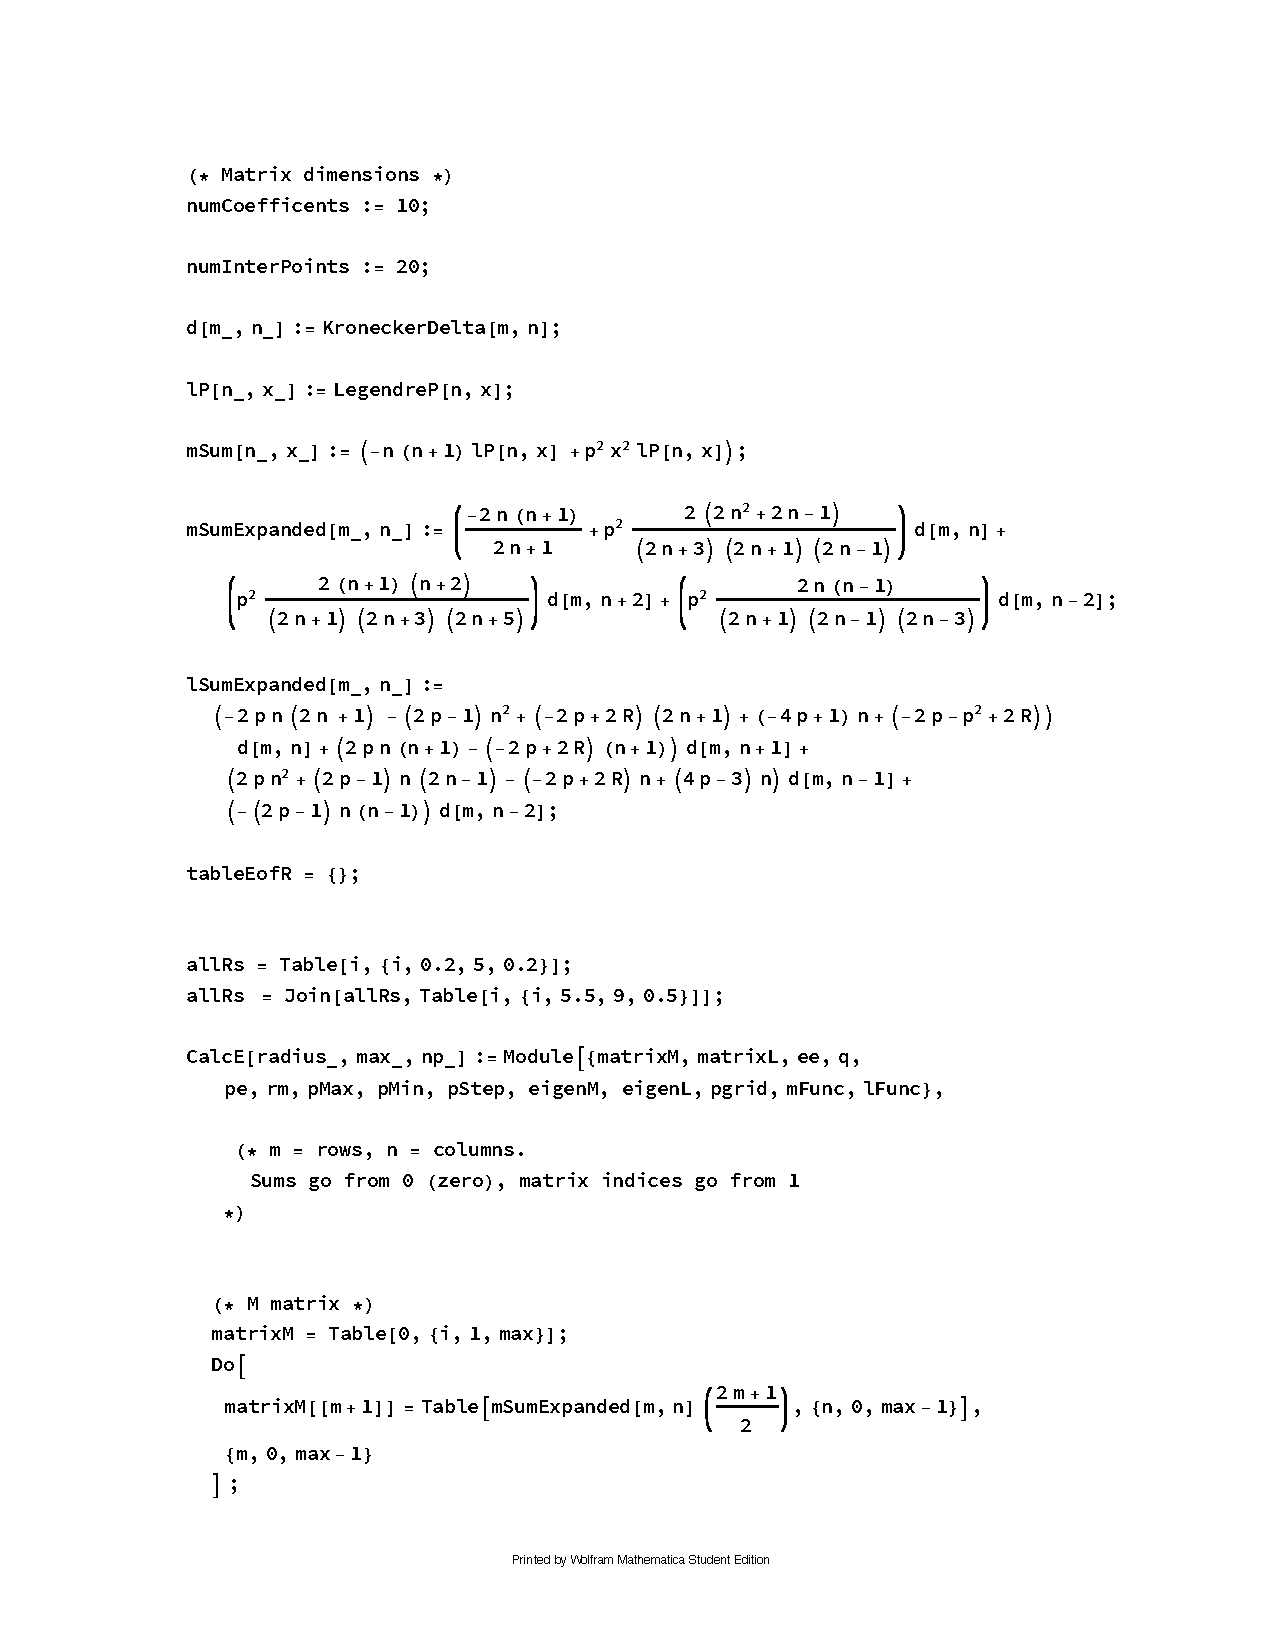
\includepdf[pages=-]{Bates-Reproduce-3D.pdf}
